
\chapter{小世界网络及影响力传播基础}
在本章中,首先介绍Kleinberg小世界网络模型和影响力传播模型,然后基于影响力传播模型介绍影响力最大化算法的相关工作。最后介绍如何用蒙特卡罗模拟估算影响力大小。

\section{Kleinberg小世界模型}
Kleinberg的小世界模型是一个由$n$个节点的集合$V$生成的随机图。
$n$个节点分布在一个$\sqrt{n} \times \sqrt{n}$的二维网格上\cite{Kleinberg2000small},为了方便,
我们把网格的上边界和下边界连接起来,同时也把网格的左边界和右边界连接起来。
这样二维网格就变成了“环面”,网格中每个节点的位置都是对称的。
网格上两个节点$u$和$v$之间的曼哈顿距离(Manhattan distance)$|uv|$是
在网格上$u$到$v$的最短路径的长度。

这个随机图上有两种类型的边:{\it 强连接}和{\it 弱连接}。
强连接是任意两个曼哈顿距离不超过$p$的节点之间生成的无向边,这里$p \geq 1$是一个模型的常数。
弱连接指连接节点$u$和网格上可能相距较远的节点$v$之间的随机边。
每个节点$u$会有$q$条互相独立的弱连接边,$u$的第$i$条弱连接边以$v$为终点的概率
正比于$1/{|uv|}^\alpha$,$\alpha\geq 0$是小世界模型的参数。
我们用$1/{|uv|}^\alpha$乘以归一化因子$\mathcal{Z} = 1/\sum_{v\in V}|uv|^{-\alpha}$(在环形网格上,这个值对于任意的节点 $u\in V$都相等),这样就得到了弱连接的概率分布函数。
最初Kleinberg描述的网络模型\cite{Kleinberg2000small}中,$u$到$v$之间的弱连接被认为是有向边,这样的网络被称为{\it 有向Kleinberg小世界网络模型}。
而有些研究工作\cite{Ghasemiesfeh2013complex}中弱连接被认为是无向的,这样的网络被称为{\it 无向Kleinberg小世界网络模型}。
两个模型在本文中都被讨论了,在分析复杂传染病的传播时,我们为了和以前的工作保持一致,
采用无向Kleinberg小世界网络模型。
分析复杂传染病的路由时,我们使用有向Kleinberg小世界网络模型。

\section{影响力传播模型}
社交网络被定义为一个有向图$G=(V,E)$,其中$V$是所有节点的集合,代表着网络中的个体,$E\subseteq V \times V$是有向边的集合。
$E$是网络中的关注或者粉丝关系,每条边也会有权值,权值代表着两个人的关系密切程度或者影响程度。
因为$G$是有向图,对于一个节点$v$,我们用$N^+(v)$表示所有$v$指向的节点集合,用$N^-(v)$表示所有指向$v$的节点集合,也就是$v$的出邻居(out-neighbours)和入邻居(in-neighbours)集合。
网络中的节点都有两种状态:{\it 未激活}(inactive)和{\it 激活}(activated)。
节点可以从未感染状态转变为感染状态,但是不能反方向转变,例如不能从已感染的状态变成未感染状态。
传播的过程可以用离散的时间步骤$0,1,2,\ldots$来描述。
在社交网络模型下,影响力传播被定义为一些疾病、信息或者想法在社交网络中沿着用户之间的有向边进行扩散。
对于一次传播过程,初始状态节点都是未激活的,选定图中的一些节点,把他们的状态设定为激活。
然后每一个时间片,按照设定的传播模型逐渐去尝试激活图未激活中的节点。
如果当前时间片没有新的节点被激活为止,传播过程结束。
接下来本文介绍常见的影响力传播模型。


\subsection{独立级联模型}
%\begin{figure}[h]
%	\centering
%	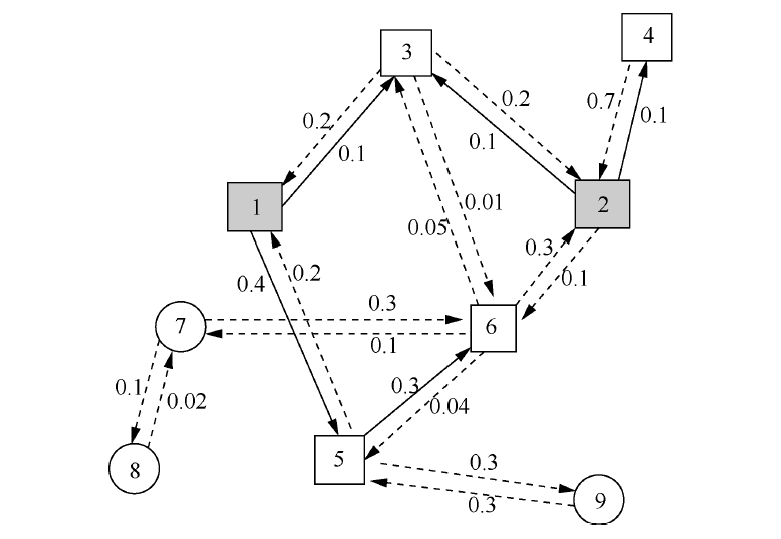
\includegraphics[width=\textwidth]{independent_cascade.png}
%	\caption{独立级联模型示意}\label{fig:independent_cascade}
%\end{figure}
独立级联模型(Independent Cascade Model)在03年被Kempe等人\cite{Kempe2003maximizing}提出,
在独立级联模型中,每条有向边$(u,v) \in E$都有一个概率值$p(u,v) \in [0,1]$代表着$v$被$u$影响的概率。
传播是随着离散时间片$t$增加而扩散的,定义$S_t$为到时间片$t$时刻为止被激活的节点的集合,定义$S_{-1}=\emptyset$。
在$t=0$时刻,选定$k$个节点$S_0$作为种子并把他们置为激活状态。
对于任意的$t\geq 1$时刻,每一个在$t-1$时刻激活的节点$v \in S_{t-1} \setminus S_{t-2}$都会对其所指向的未激活节点
$u \in N^+(u) \setminus S_{t}$进行一次激活尝试,成功激活$u$的概率是$p(v,u)$,不同节点之间的激活尝试相互独立。
如果节点$u$在某次激活尝试中被激活,则$u$在$t$时刻被激活。
如果$S_{t-1} \setminus S_{t-2}$中所有节点对$u$的尝试都失败,则$u$在$t$时刻未被激活。
当某一时刻没有节点被激活时,传播终止。

图\ref{fig:independent_cascade}给出了独立级联模型下的一次传播过程,图中的虚线边表示一次失败的激活尝试,实线表示成功的激活尝试。
在$t=0$时刻节点1和节点2被选为种子,在$t=1$的时刻,节点1和节点2成功激活了节点3、4、5,节点2对节点6的激活尝试失败。
在$t=2$时刻节点5成功激活了节点6,节点3和4发出的尝试激活失败。
在$t=3$时刻节点6没有激活任何节点,传播过程终止,最后被影响的节点集合是$\{1,2,3,4,5,6\}$。

\subsection{线性阈值模型}
独立级联模型(Linear Threshold Model)\cite{Kempe2003maximizing}描述的传播过程中,节点对节点的作用是互相独立的,而且每个节点只需要一次成功的激活尝试就能被激活。
而在有些场景中,一个节点的激活需要多个节点的共同作用,像购物或者接受新商品等。
为了描述类似举要多个节点累计作用才能激活的场景,线性阈值模型被提出来。

在现行与之模型中,每条有向边$(u,v) \in E$都被赋予了一个权重$w(u,v)$,对于每个节点来说,所有指向它的边权重之和不超过$1$。
也就是$\sum_{u \in N^-(u)} w(u,v) \leq 1$。
每个节点$v$还有自己的阈值$\theta_v \in [0,1]$,在传播开始前,每个节点独立的在$[0,1]$中依据均匀分布选择自己的阈值。
在每个时间节点$t \geq 1$,对于所有还没被激活的节点$v \in V \setminus S_{t-1}$,
如果由已激活节点发出的指向$v$的的有向边权重之和大于$v$的阈值,也就是$\sum_{u \in N^-(u) \cap S_{t-1}} w(u,v) \geq \theta_v$,
则$v$会在$t$时刻被激活,否则停留在未激活状态。
同样,当在某一时刻没有新节点被激活时,传播停止。

\subsection{通用级联模型}
独立级联模型的假设过强,于是Kempe\cite{Kempe2003maximizing}提出了通用级联模型(General Cascade Model),
这是独立级联模型的一般形式。
对于通用级联模型,每个节点$v$有个激活函数$p_v(u,S):N^-(v) \times 2^{N^-(v)} \to [0,1]$,
这里$S \subset N^-(v)$并且$u \in N^-(v) \setminus S$。
传播过程整体和独立级联模型一致,
在$t=0$时刻选定种子节点后,在$t \geq 1$的时间片,
对于尚未激活的节点$v \not\in S_{t-1}$,把$v$刚刚激活的的入邻居$N^-(v) \cap (S_{t-1}\setminus S_{t-2})$按照$u_1,u_2,\dots,u_{\ell}$排列,
依据这个顺序依次尝试激活节点$v$。
如果$u_1,u_2,\dots,u_{i-1}$没有成功激活$v$,则令$S = (N^-(v) \cap S_{t-2}) \cup \{u_1,u_2,\dots,u_{i-1}\}$
然后$u_{i}$以$p_v(u_i,S)$的概率尝试激活$v$。
在通用级联模型中,$p_v(u,S)$满足顺序无关性质,也就是最终$u_1,u_2,\dots,u_{\ell}$尝试激活$v$之后$v$被激活的概率
与这$\ell$次尝试的顺序无关,只与尝试激活的节点集合有关。
注意到独立级联模型是通用级联模型的特例,只需要令$p_v(u,S)$恒等于$p(u,v)$即可。


\subsection{通用阈值模型}
在通用阈值模型中(General Threshold Model),每个节点$v$有一个阈值函数$f_v:2^{N^-(v)} \to [0,1]$。
阈值函数$f_v$是单调非减(monotone)而且$f_v(\emptyset)=0$。
和线性阈值模型相同,在传播开始前,每个节点独立的在$[0,1]$中依据均匀分布选择自己的阈值。
然后在接下来的每一时刻$t\geq 1$,对于$v \not\in S_{t-1}$,
如果$f_v(S_{t-1} \cap N^-(v)) \geq \theta_v$,
节点$v$被激活,否则节点$v$保持未激活状态。

%线性阈值模型是通用阈值模型的特例,只需要令$f_v(S) = \sum_{u\in S}w(u,v)$。
通用阈值模型和通用级联模型也是等价的,给定阈值函数$f_v$,可以得到激活函数
$p_v(u,S) = \frac{f_v(S \cup \{u\}) - f_v(S)}{1-f_v(S)}$。
给定激活函数$p_v$,同样可以得到对应的通用阈值模型的阈值函数
$f_v(S) = 1 - \Pi_{i=1}^{\ell}(1-p_v(u_i, \{u_1,u_2,\dots,u_{i-1}\}))$。


\section{影响力最大化问题}
在一个$n$个节点的图中,给定影响力传播模型,最多经过$n-1$步,传播就会结束。
我们称以$S_0$为种子集合最终传播停止时被影响的节点集合是$\Phi(S_0)$。
$\Phi(S_0)$是一个依赖于影响力传播过程的随机集合。
影响力最大化问题就是在给定种子数量选择合适的种子集合的情况下最大化$\Phi(S_0)$的期望大小。
我们定义$\sigma(S_0) = \mathbb{E}(\Phi(S_0))$,$\sigma(\cdot)$就被称作为{\it 影响力函数}。
通常所研究的种子集合大小不超过$k$的影响力最大化问题可以公式化为$S^* = \mathrm{argmax}_{S \in V, |S|=k} \sigma(S)$,
$S^*$为最优解集合。
通常选用的影响力模型是独立级联模型或者线性阈值模型,近些年来也有很多基于这两个传播模型的影响力最大化算法被提出。

影响力最大化本质上描述了社交网络中的营销(Social marketing)问题,
有新的产品或者广告发布时,希望选择人试用并转发消息,然后口口相传最后扩散到很多人。
商家最后的目的就是希望可以遭到影响力最大的用户集合使得最终扩散的范围最大,这也就是影响力最大化的目标。
影响力最大化问题是社交网络中营销问题的抽象,研究影响力最大化问题对于商家试用品和广告的投放有很大帮助。
下面介绍一下影响力最大化问题的常见算法。

\subsection{贪心算法}
影响力最大化问题的复杂度很高,至少比集合覆盖最大化(Max Set Cover)问题要难,而集合覆盖最大化问题是NP-Hard的。
但是影响力函数$\sigma(\cdot)$在独立级联模型和线性阈值模型下被证明是次模的\cite{Kempe2003maximizing}。
次模函数是定义在集合函数上的,对于一个集合函数$f:2^V \to \mathbb{R}$,
如果对于任意的输入集合$S \subseteq T \subseteq V$和元素$u \in V \setminus T$都有
$f(S \cup \{u\}) - f(S) \geq f(T \cup \{u\}) - f(T)$,
则称函数$f$满足次模(submodular)性质。
次模性质本质上是边际效益递减,同样加入一个元素$u$,$f(T)$函数值的提升不如$f(S)$的提升大。
如果对于输入$S \subseteq T \subseteq V$,$f$函数还满足$f(S) \leq f(T)$,则称函数$f$是单调非减的。
对于单调非减和次模的函数$f$,贪心算法可以做到$1-\frac{1}{e}$的近似比。
对于影响力最大化问题,由于影响力函数$\sigma(\cdot)$是单调和次模的,可以调用贪心算法解决。
然而每一步$\sigma(S)$的计算是$\#$P-Hard的,不能精确求解。
通常采用蒙特卡洛模拟方法来估算影响力,随机模拟10000次传播过程,取被激活节点个数的期望作为影响力。
由于蒙特卡罗模拟是近似得到影响力大小,贪心算法最后可以取得$1-\frac{1}{e}-\varepsilon$的近似比。
蒙特卡洛贪心算法执行过程如Algorithm \ref{alg:submodular_greed}所示。

\begin{algorithm}
	\caption{\textbf{MC-Greedy(G,k)}: Monte Carlo greedy for influence maximization.}
	\label{alg:mc_greed} 
	\begin{algorithmic}[1]
		\Require $G$: social graph of IC or LT model, $k$: budget of seeds.
		\Ensure selected seed set $S$.
		\State Initialize $S = \emptyset$
		\For {$i=1$ to $k$}
			\State $v = \mathrm{argmax}_{u \in V \setminus S}$ \Call{MC-Spread}{$S \cup \{u\}, G$}
			\State $S = S \cup \{u\}$
		\EndFor
		\State \Return $S$
		\Function{MC-Spread}{$S$, $G$}
			\State $count=0$
			\For {$j=1$ to $R$}
				\State simulate diffusion process on graph $G$ with seed set $S$
				\State $n\_spread \gets$ the number of active nodes
				\State $count = count + n\_spread$
			\EndFor
			\State \Return $count/R$
		\EndFunction
	\end{algorithmic} 
\end{algorithm}

\subsection{CELF算法}
暴力的贪心算法时间复杂度很高,对于$k$个种子的影响力最大化问题,需要迭代$k$轮,每一轮需要便利每一个种子,利用蒙特卡洛模拟估计影响力大小。
最终需要的时间复杂度为$O(Rknm)$,$R$是蒙特卡洛模拟需要的传播模拟次数。对于几万个节点的图,贪心算法的运行时间可能就需要几周。
Leskovec等人\cite{Leskovec2007celf}基于次模问题优化中的lazy evaluation方法,优化了暴力的贪心算法,得到了近700倍的算法性能提升。
定义函数的差分为$\Delta_u f(S) = f(S \cup \{u\}) - f(S)$,其中$u \not\int S$。
对于单调次模函数$f$和集合$S \subseteq T \subseteq V$来说,有$\Delta_u f(S) \geq \Delta_u f(T)$。
在蒙特卡洛贪心算法中,每一轮都需要计算每个节点$v$的$\Delta_v f(S)$然后选出提升最大的节点加入$S$。
设$S_i$为第$i$轮为止选择到的种子节点集合,如果在第$i$轮算法运行中,发现存在节点$u,v \not\in S_{i-1}$,而且$\Delta_u f(S_{i-2}) \leq \Delta_v f(S_{i-1})$。
那么由次模性质可以得到$u$在第$i$轮的提升一定会小于$v$,所以不会被选为种子,在第$i$轮$u$的影响力提升就没有必要再计算。
所以加入一个结构存储之前计算的影响力提升,可以减少对影响力的重复估算,极大提升算法效率。
CELF算法就是利用这个思想,通过优先队列实现。

\begin{algorithm}
	\caption{\textbf{CELF(G,k)}: accelerated greedy algorithm with lazy evaluation.}
	\label{alg:celf} 
	\begin{algorithmic}[1]
		\Require $G$: social graph of IC or LT model, $k$: budget of seeds.
		\Ensure selected seed set $S$.
		\State Initialize $S = \emptyset$, priority queue $Q = \emptyset$
		\ForAll {$v$ in V}
			\State $v.margin \gets$ \Call{MC-Spread}{$\{v\}, G$}
			\State $v.iteration = 1$
			\State insert element $v$ into $Q$ with $v.margin$ as the key
		\EndFor
		\State $iteration = 1, spread = 0$
		\While{$iteration \leq k$}
			\State extract top (max) element $v$ of $Q$
			\If{$v.iteration == iteration$}
				\State $S = S \cup \{u\}$
				\State $iteration = iteration+1$
				\State $spread = spread + v.margin$
			\Else
				\State $v.margin \gets$ \Call{MC-Spread}{$S \cup \{v\}, G$} - $spread$
				\State re-insert $v$ into $Q$
			\EndIf
		\EndWhile
		\State \Return $S$
	\end{algorithmic} 
\end{algorithm}

\subsection{PMIA算法}
MC-Greedy算法和CELF算法还是通过蒙特卡洛模拟来估算集合的影响力大小。陈卫等人提出了一个启发式算法,近似的估算影响力,再次提升了算法的性能,同时算法的效果能够媲美贪心算法。
PMIA算法\cite{chen2010sharpphard}中,利用比较容易计算的树状图来避免了蒙特卡洛模拟。
核心子算法是Maximum Influence Arborescence(MIA),PMIA算法对于每一个节点$v$构建了以$v$为根的局部树状结构,
然后在局部的树状结构上可以用动态规划高效计算影响力。
因为影响力传播衰减很快,而且估算整体的影响力很难,局部树状结构也是合理的。
PMIA算法同时也根据树状结构设计了线性更新影响力提升值的方法,在加入新的种子节点后很快更新每个节点的影响力。
原算法的整体过程比较复杂,由多个子算法构成,这里不再赘述。

\subsection{TIM算法}
基于蒙特卡洛模拟的贪心算法速度较慢,启发式算法速度较快但是没有理论的近似比保证。
Borgs等人\cite{borgs2014rrset}在14年提出了基于逆向可达集合(Reverse Reachable Set)的近线性算法,同时也有基于最大集合覆盖的$1-\frac{1}{e}$的近似比保证。
算法的核心思想是做逆向蒙特卡洛模拟,把图中每条有向边反向,沿着反向的边做传播。
算法会随机的选择图中的节点$v$,然后以$v$为根节点做反向蒙特卡洛模拟,传播过程中激活的节点称为$v$的逆向可达集合,多次模拟得到多个逆向可达集合。
Borgs等人证明了,给定种子集合$S$,$v$被激活的概率就是$S$和$v$的逆向可达集合有交集的概率。
因此可以随机从途中选择节点,产生逆向可达集合,多次实验之后生成很多逆向可达集合。
给定一个种子集合,影响力大小正比于种子集合与多少个多逆向可达集合有交集,这就转变为最大集合覆盖问题,可以用贪心很快求解。
随后Tang等人\cite{tang2014newrrset}工程上实现了这个算法(TIM算法),并测试了算法在上亿节点的效果和运行时间。该算法已经能处理Twitter这种级别的社交网络。
在求解最大覆盖问题时,依据逆向可达集合简历倒排索引,维护每个节点覆盖的逆向可达集合,每次贪心的选择覆盖最多逆向可达集合的节点加入种子节点。

\begin{algorithm}
	\caption{\textbf{TIM(G,k)}: Two-phase Influence Maximization.}
	\label{alg:tim} 
	\begin{algorithmic}[1]
		\Require $G$: social graph of IC or LT model, $k$: budget of seeds.
		\Ensure selected seed set $S$.
		\State Initialize $S = \emptyset$, $\mathcal{R} = \emptyset$
		\State compute the the number of RRsets needed $\theta$
		\For {$i=1$ to $\theta$}
			\State randomly pick a node $v$ from $V$
			\State generate RRset $R_v$ for $v$
			\State insert $R_v$ into $\mathcal{R}$
		\EndFor
		\State build reverse index $Idx$ of $\mathcal{R}$
		\For {$i=1$ to $k$}
			\State fetch $v$ that has max degree from $Idx$
			\State insert $v$ into $S$
			\State update $Idx$
		\EndFor
		\State \Return $S$
	\end{algorithmic} 
\end{algorithm}

\section{本章小结}
本章主要介绍了本文使用的Kleinberg小世界模型以及影响力传播模型和影响力最大化算法等概念,并给出了精确的数学定义。
2.1节介绍了Kleinberg的小世界模型,主要分析了弱连接的生成方式。
2.2节介绍了影响力传播模型,重点介绍了线性阈值模型和独立级联模型以及他们的通用形式。
2.3节介绍了基于线性阈值模型或者独立级联模型和影响力最大化,影响力最大化算法在近些年来被许多学者研究,很多近似算法和启发式算法被提出。


